\documentclass[11pt]{article}
\usepackage[margin=1in]{geometry}
\usepackage[T1]{fontenc}
\usepackage{lmodern}
\usepackage{amsmath,amssymb,amsthm}
\usepackage{tikz,tikz-cd,needspace}
\usepackage[hidelinks]{hyperref}
\usetikzlibrary{arrows.meta,patterns}

\theoremstyle{definition}
\newtheorem{Def}{Definition}
\newtheorem{Ex}{Example}
\theoremstyle{remark}
\newtheorem{Rmk}{Remark}
\DeclareMathOperator{\ev}{ev}
\DeclareMathOperator{\ord}{ord}
\DeclareMathOperator{\divisor}{div}
\DeclareMathOperator{\Spec}{Spec}
\DeclareMathOperator{\Cl}{Cl}
\DeclareMathOperator{\Pic}{Pic}
\DeclareMathOperator{\Bl}{Bl}
\DeclareMathOperator{\Conv}{conv}
\DeclareMathOperator{\Cone}{Cone}
\newcommand{\Sg}{\Sigma}
\newcommand{\sg}{\sigma}
\newcommand{\cO}{\mathcal{O}}
\newcommand{\set}[1]{\left\{#1\right\}}
\newcommand{\braket}[2]{\left\langle #1,#2\right\rangle}
\newcommand{\bA}{\mathbb{A}}
\newcommand{\bP}{\mathbb{P}}
\newcommand{\bR}{\mathbb{R}}
\newcommand{\bN}{\mathbb{N}}
\newcommand{\bZ}{\mathbb{Z}}
\newcommand{\bC}{\mathbb{C}}
\newcommand{\bQ}{\mathbb{Q}}
\newcommand{\bF}{\mathbb{F}}
\newcommand{\vf}{\varphi}
\newcommand{\x}{\times}
\newcommand{\isom}{\cong}
\renewcommand{\figurename}{Diagram}


\begin{document}

\begin{center}
    {\Large\bfseries October 19, 2026}
\end{center}

\section{Recall: sections, rational functions, and projective maps}

Work over \(\bC\). Sections of a line bundle \(L\to X\) are geometric
objects: a section chooses one vector in each fiber. They become
easier to calculate with after choosing a nonzero rational section
\(s_D\). If \(\divisor(s_D)=D\), then every rational section has a
unique expression
\[
    \widetilde{s}=f s_D,\qquad f\in\bC(X),
\]
and it is regular precisely when
\[
    \divisor(f)+D\geq0.
\]
Thus a regular section can be represented by a rational function with
poles: the zeros of the chosen reference section compensate for them.

% First photograph, left column: the bundle and a section's zero divisor.
\begin{figure}[htbp]
    \centering
    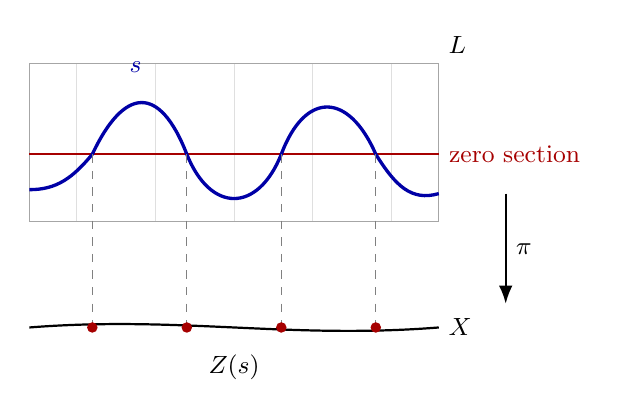
\begin{tikzpicture}[x=1cm,y=1cm,>=Latex,font=\small]
        \draw[gray!70] (-2.6,1.35) rectangle (2.6,3.35);
        \foreach \a in {-2,-1,0,1,2}
            \draw[gray!25] (\a,1.35)--(\a,3.35);
        \draw[red!65!black,thick] (-2.6,2.2)--(2.6,2.2)
            node[right] {zero section};
        \draw[blue!65!black,very thick]
            (-2.6,1.75) .. controls (-2.25,1.75) and (-2.05,1.9) .. (-1.8,2.2)
            .. controls (-1.4,3.05) and (-0.95,3.1) .. (-0.6,2.2)
            .. controls (-0.3,1.45) and (0.3,1.45) .. (0.6,2.2)
            .. controls (0.9,3) and (1.45,3) .. (1.8,2.2)
            .. controls (2.05,1.8) and (2.25,1.6) .. (2.6,1.7);
        \node[blue!65!black] at (-1.25,3.3) {$s$};
        \node[above right] at (2.6,3.35) {$L$};
        \draw[thick] (-2.6,0) .. controls (-0.7,0.15) and (0.7,-0.15) .. (2.6,0);
        \node[right] at (2.6,0) {$X$};
        \foreach \a in {-1.8,-0.6,0.6,1.8} {
            \draw[dashed,gray] (\a,2.2)--(\a,0);
            \fill[red!65!black] (\a,0) circle (1.9pt);
        }
        \draw[->,thick] (3.45,1.7)--(3.45,0.3)
            node[midway,right] {$\pi$};
        \node[below] at (0,-0.22) {$Z(s)$};
    \end{tikzpicture}
    \caption{A schematic regular section \(s\). Its intersections with the
    zero section project to its zero divisor \(Z(s)\) on \(X\).
    The picture illustrates the regular case; a rational reference section
    may also have poles.}
    \label{fig:oct19-diagram1}
\end{figure}

\subsection{Three descriptions of the same projective coordinates}

Suppose \(s_0,\ldots,s_r\) are global sections of \(L\). At a point \(x\)
where they do not all vanish, their values lie in the same
one-dimensional vector space \(L|_x\), so they determine
\[
    \vf(x)=[s_0(x):\cdots:s_r(x)]\in\bP^r.
\]
Changing the identification \(L|_x\isom\bC\) rescales every coordinate
by the same scalar. In terms of rational functions,
\[
    s_i=f_i s_D
    \quad\Longrightarrow\quad
    \vf=[f_0:\cdots:f_r]
\]
where this rational-function formula can be evaluated. On the open set
\(s_j\ne0\), the regular affine coordinates are instead
\[
    \left(\frac{s_0}{s_j},\ldots,\widehat{\frac{s_j}{s_j}},
          \ldots,\frac{s_r}{s_j}\right).
\]
The hat means that the coordinate equal to \(1\) is omitted.
These are equivalent descriptions, provided one keeps track of the
chosen frame and of where the denominator does not vanish. A line
bundle is basepoint free when its full space of global sections has
no common zero.

\section{Dividing by a section translates the polytope}

For a torus-invariant Cartier divisor \(D\) on \(X_\Sg\), write
\[
    L=\cO_{X_\Sg}(D),\qquad
    P_D=\set{m\in M_\bR:
       \braket{m}{u_\rho}\geq-a_\rho\text{ for all }\rho}.
\]
The global monomial sections are
\[
    s_m=\chi^m s_D,\qquad m\in P_D\cap M.
\]
The lattice points describe sections regular \emph{everywhere} on
\(X_\Sg\), not merely on a single affine chart.

% The notes call this a trapezoid and refer back to October 16.
% Use that same polygon; the calculation at (2,0) also applies to 2H-E.
We return to the trapezoid from October 16:
\[
    P=\Conv\{(0,0),(2,0),(1,1),(0,1)\}
      =\set{(r,q):r,q\geq0,\ q\leq1,\ r+q\leq2}.
\]
Its five lattice points give
\[
    \vf_P:(\bC^\times)^2\longrightarrow\bP^4,\qquad
    (s,t)\longmapsto[1:s:t:s^2:st].
\]
In this example the map extends to an embedding of the normal-fan
variety, as the chart calculations from October 16 showed.
The point of today's discussion is why that conclusion requires a check.

% First photograph, second column: the polygon and its normal fan.
\begin{figure}[htbp]
    \centering
    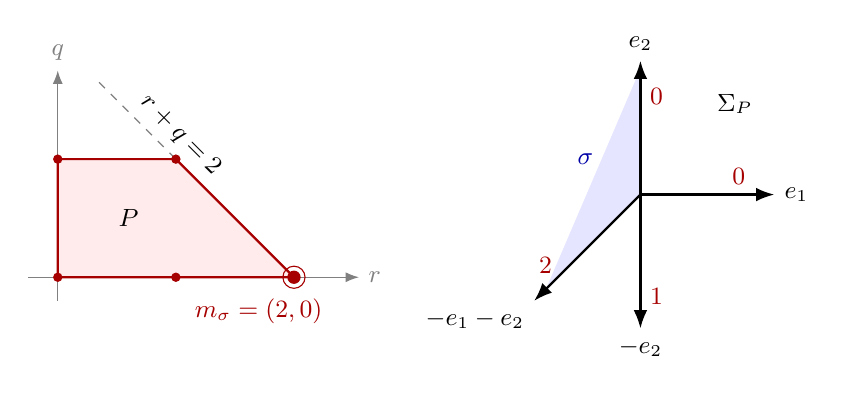
\begin{tikzpicture}[>=Latex,font=\small]
        \begin{scope}[x=1.5cm,y=1.5cm]
            \draw[->,gray] (-0.25,0)--(2.55,0) node[right] {$r$};
            \draw[->,gray] (0,-0.2)--(0,1.75) node[above] {$q$};
            \fill[red!8] (0,0)--(2,0)--(1,1)--(0,1)--cycle;
            \draw[red!65!black,thick] (0,0)--(2,0)--(1,1)--(0,1)--cycle;
            \draw[dashed,gray] (0.35,1.65)--(1,1);
            \node[above right,rotate=-45] at (0.55,1.45) {$r+q=2$};
            \foreach \p in {(0,0),(1,0),(0,1),(1,1)}
                \fill[red!65!black] \p circle (1.7pt);
            \fill[red!65!black] (2,0) circle (2.4pt);
            \draw[red!65!black] (2,0) circle (4pt);
            \node[below,red!65!black] at (1.7,-0.1) {$m_\sigma=(2,0)$};
            \node at (0.6,0.5) {$P$};
        \end{scope}
        \begin{scope}[shift={(7.4,1.05)},x=1cm,y=1cm]
            \fill[blue!10] (0,0)--(0,1.6)--(-1.2,-1.2)--cycle;
            \draw[->,thick] (0,0)--(1.7,0) node[right] {$e_1$};
            \draw[->,thick] (0,0)--(0,1.7) node[above] {$e_2$};
            \draw[->,thick] (0,0)--(-1.35,-1.35)
                node[below left] {$-e_1-e_2$};
            \draw[->,thick] (0,0)--(0,-1.7) node[below] {$-e_2$};
            \node[red!65!black,above] at (1.25,0) {$0$};
            \node[red!65!black,right] at (0,1.25) {$0$};
            \node[red!65!black,left] at (-1,-0.9) {$2$};
            \node[red!65!black,right] at (0,-1.3) {$1$};
            \node[blue!65!black] at (-0.7,0.45) {$\sigma$};
            \node at (1.2,1.15) {$\Sigma_P$};
        \end{scope}
    \end{tikzpicture}
    \caption{The trapezoid \(P\) and its inward normal fan.
    The red numbers on the rays are the divisor coefficients \(a_\rho\).
    The shaded cone \(\sigma=\Cone(e_2,-e_1-e_2)\) corresponds to
    the marked vertex \(m_\sigma=(2,0)\).}
    \label{fig:oct19-diagram2}
\end{figure}

\subsection{The local frame on an affine chart}

For a maximal cone \(\sigma\), the Cartier datum \(m_\sigma\) satisfies
\[
    \braket{m_\sigma}{u_\rho}=-a_\rho
    \qquad(\rho\subseteq\sigma).
\]
The section
\[
    e_\sigma=\chi^{m_\sigma}s_D
\]
is a nowhere-vanishing frame on the affine chart \(X_\sigma\).
Consequently,
\[
    H^0(X_\sigma,L)\ \xrightarrow{\ \widetilde{s}\mapsto
                  \widetilde{s}/e_\sigma\ }\ \cO(X_\sigma)
\]
is an isomorphism of \(\cO(X_\sigma)\)-modules.
For a monomial section this becomes
\[
    \boxed{\frac{s_m}{e_\sigma}=\chi^{m-m_\sigma}.}
\]
Thus dividing sections by the distinguished local frame means
subtracting \(m_\sigma\) from every exponent.

% First photograph, lower middle: a line bundle over the affine chart.
\begin{figure}[htbp]
    \centering
    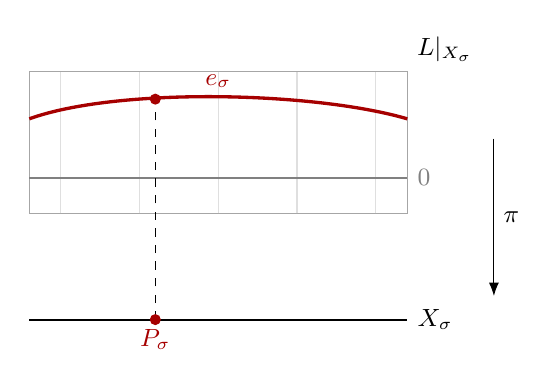
\begin{tikzpicture}[x=1cm,y=1cm,>=Latex,font=\small]
        \draw[gray!70] (-2.4,1.35) rectangle (2.4,3.15);
        \foreach \a in {-2,-1,0,1,2}
            \draw[gray!25] (\a,1.35)--(\a,3.15);
        \draw[gray,thick] (-2.4,1.8)--(2.4,1.8)
            node[right] {$0$};
        \draw[red!65!black,very thick]
            (-2.4,2.55) .. controls (-1.3,2.95) and (1.2,2.9) .. (2.4,2.55);
        \node[above,red!65!black] at (0,2.82) {$e_\sigma$};
        \node[above right] at (2.4,3.15) {$L|_{X_\sigma}$};
        \draw[thick] (-2.4,0)--(2.4,0) node[right] {$X_\sigma$};
        \draw[dashed] (-0.8,0)--(-0.8,2.8);
        \fill[red!65!black] (-0.8,0) circle (2pt)
            node[below] {$P_\sigma$};
        \fill[red!65!black] (-0.8,2.8) circle (2pt);
        \draw[->] (3.5,2.3)--(3.5,0.3) node[midway,right] {$\pi$};
    \end{tikzpicture}
    \caption{The local frame \(e_\sigma\) never meets the zero section.
    It identifies \(L|_{X_\sigma}\) with \(X_\sigma\x\bA^1\);
    dividing by it turns a regular section into a regular function.}
    \label{fig:oct19-diagram3}
\end{figure}

In the trapezoid example, \(m_\sigma=(2,0)\), so \(e_\sigma=s^2s_D\).
Dividing the five global sections by this frame gives
\[
    (s^{-2},s^{-1},t/s^2,1,t/s).
\]
The section indexed by \(m_\sigma\) becomes the constant \(1\).
This is the section that does not vanish at the fixed point
\(P_\sigma\).

\subsection{The dual cone records all local regular monomials}

Translation puts the vertex at the origin, and
\[
    P-m_\sigma\subseteq\sigma^\vee
      =\Cone\bigl((-1,0),(-1,1)\bigr)
      =\set{(a,b):b\geq0,\ a+b\leq0}.
\]
The affine chart is
\[
    X_\sigma=\Spec\bC[\sigma^\vee\cap M],
\]
so the lattice points of the \emph{whole cone} index its regular
monomials. In this case, every such lattice point has the expression
\[
    (a,b)=(-a-b)(-1,0)+b(-1,1).
\]
The two generators form a lattice basis, and hence
\[
    \bC[\sigma^\vee\cap M]=\bC[s^{-1},t/s].
\]
With \(\xi=s^{-1}\) and \(\eta=t/s\), the normalized affine tuple is
\[
    (\xi^2,\xi,\xi\eta,\eta),
\]
which identifies the image chart with \(X_\sigma\isom\bA^2\).

% First photograph, lower right: the translated polygon in the dual cone.
\begin{figure}[htbp]
    \centering
    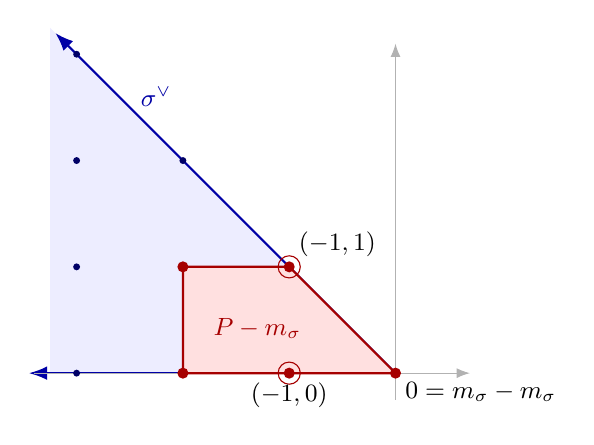
\begin{tikzpicture}[x=1.35cm,y=1.35cm,>=Latex,font=\small]
        \fill[blue!7] (0,0)--(-3.25,0)--(-3.25,3.25)--cycle;
        \draw[->,blue!65!black,thick] (0,0)--(-3.45,0);
        \draw[->,blue!65!black,thick] (0,0)--(-3.2,3.2);
        \draw[->,gray!60] (0,-0.25)--(0,3.1);
        \draw[->,gray!60] (-3.4,0)--(0.7,0);
        \foreach \a in {-3,-2,-1,0}
            \foreach \b in {0,1,2,3} {
                \pgfmathtruncatemacro{\inside}{(\a+\b<=0)}
                \ifnum\inside=1
                    \fill[blue!40!black] (\a,\b) circle (1.25pt);
                \fi
            }
        \fill[red!12] (-2,0)--(0,0)--(-1,1)--(-2,1)--cycle;
        \draw[red!65!black,thick] (-2,0)--(0,0)--(-1,1)--(-2,1)--cycle;
        \foreach \p in {(-2,0),(-1,0),(0,0),(-2,1),(-1,1)}
            \fill[red!65!black] \p circle (2pt);
        \draw[red!65!black] (-1,0) circle (4pt);
        \draw[red!65!black] (-1,1) circle (4pt);
        \node[below] at (-1,0) {$(-1,0)$};
        \node[above right] at (-1,1) {$(-1,1)$};
        \node[below right] at (0,0) {$0=m_\sigma-m_\sigma$};
        \node[red!65!black] at (-1.3,0.42) {$P-m_\sigma$};
        \node[blue!65!black] at (-2.25,2.6) {$\sigma^\vee$};
    \end{tikzpicture}
    \caption{Dividing monomials by \(\chi^{m_\sigma}\) translates \(P\) into
    \(\sigma^\vee\). Red points come from global monomial sections.
    All cone lattice points give local regular functions; the two circled
    nonzero points generate their semigroup.}
    \label{fig:oct19-diagram4}
\end{figure}

This answers the question about the dots. Points of \(P-m_\sigma\)
come from global sections after dividing by the frame. The extra cone
points give local functions, but multiplying them by the frame need
not produce sections regular on every other chart. For example,
\(s^{-3}\) is regular on \(X_\sigma\), whereas
\[
    s^{-3}e_\sigma=s^{-1}s_D
\]
is not a global section, since \((-1,0)\notin P\).
The variety is denoted \(X_\sigma\); \(\sigma^\vee\) describes its
coordinate ring, not a different chart \(X_{\sigma^\vee}\).

\section{Ample does not always mean very ample}

A full-dimensional lattice polytope \(P\subseteq M_\bR\) determines
an inward normal fan \(\Sigma_P\), a normal projective toric variety
\(X_{\Sigma_P}\), and an ample Cartier divisor \(D_P\). Its lattice
points give a basepoint-free complete linear system, but the map
\[
    \vf_{D_P}:X_{\Sigma_P}\longrightarrow
       \bP^{|P\cap M|-1}
\]
need not be a closed embedding.

The chart calculation explains the additional requirement. At a vertex
\(v\), the normalized sections have exponents \(m-v\). To recover the
entire affine chart, they must generate its semigroup:
\[
    \bN\set{m-v:m\in P\cap M}
       =\Cone(P-v)\cap M.
\]
Here \(\bN\set{\cdots}\) means all nonnegative integral combinations.
It is not enough that the vectors generate the same real cone.
Checking this equality at every vertex is the vertex-chart criterion
for very ampleness.

In dimension two every lattice polygon satisfies this condition
(indeed, every lattice polygon is normal). Thus its associated divisor
is very ample. The next example shows what can go wrong in dimension
three. Smoothness of the variety is a separate issue from whether a
given linear system embeds it.

\section{A three-dimensional example}

Put \(M=\bZ^3\), let \(e_1,e_2,e_3\) be its standard basis, and set
\[
    w=(1,1,2),\qquad
    P=\Conv\{0,e_1,e_2,w\}.
\]
This is the height-two Reeve tetrahedron. Its only lattice points
are its four vertices.

% Diagram 5: the Reeve tetrahedron of height two.
\begin{figure}[htbp]
    \centering
    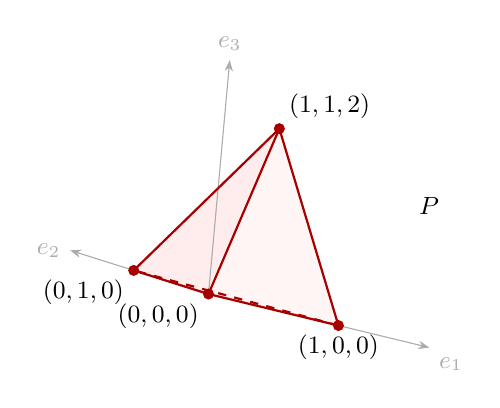
\begin{tikzpicture}[
        x={(1.65cm,-0.40cm)},y={(-0.95cm,0.30cm)},z={(0.10cm,1.10cm)},
        font=\small,line join=round,
        >={Stealth[length=4pt]}
    ]
        \coordinate (O) at (0,0,0);
        \coordinate (A) at (1,0,0);
        \coordinate (B) at (0,1,0);
        \coordinate (C) at (1,1,2);
        \fill[red!4] (O)--(A)--(C)--cycle;
        \fill[red!7] (O)--(B)--(C)--cycle;
        \draw[->,gray!65] (O)--(1.70,0,0) node[below right] {$e_1$};
        \draw[->,gray!65] (O)--(0,1.85,0) node[left] {$e_2$};
        \draw[->,gray!65] (O)--(0,0,2.70) node[above] {$e_3$};
        \draw[red!65!black,thick,dashed] (A)--(B);
        \draw[red!65!black,thick] (O)--(A)--(C)--(B)--cycle;
        \draw[red!65!black,thick] (O)--(C);
        \foreach \point in {O,A,B,C}
            \fill[red!65!black] (\point) circle (2pt);
        \node[below left] at (O) {$(0,0,0)$};
        \node[below] at (A) {$(1,0,0)$};
        \node[below left] at (B) {$(0,1,0)$};
        \node[above right] at (C) {$(1,1,2)$};
        \node at (1.60,0,1.60) {$P$};
    \end{tikzpicture}
    \caption{The tetrahedron
    \(P=\operatorname{conv}\{(0,0,0),(1,0,0),(0,1,0),(1,1,2)\}\).
    Its four vertices are its only lattice points. The dashed edge is hidden
    by the two shaded faces.}
    \label{fig:oct19-diagram5}
\end{figure}

The lattice-point map is
    \[
    \vf_P:(\bC^\times)^3\longrightarrow\bP^3,\qquad
    (s,t,u)\longmapsto[1:s:t:stu^2].
\]
Since
\[
    \vf_P(s,t,u)=\vf_P(s,t,-u),
\]
it is not injective. In fact its image is the entire dense torus of
\(\bP^3\): for any nonzero \(a,b,c\), choose \(u\) with
\(u^2=c/(ab)\). Therefore
\[
    \boxed{\overline{\vf_P(T)}=\bP^3.}
\]
The equality that fails is the identification of this image with
\(X_{\Sigma_P}\) for the prescribed lattice \(M=\bZ^3\).
The exponent differences generate only
\[
    M'=\bZ e_1+\bZ e_2+\bZ w
       =\set{(a,b,c)\in\bZ^3:c\text{ is even}},
\]
an index-two sublattice of \(M\). The induced morphism
\(X_{\Sigma_P}\to\bP^3\) is finite of degree two. It is not an
embedding, and it is not a normalization map: \(\bP^3\) is already
normal.

\subsection{The missing local monomial and the singular chart}

At the vertex \(0\), the lattice point
\[
    h=(1,1,1)=\tfrac12(e_1+e_2+w)
\]
lies in \(\Cone(P)\), but not in the semigroup generated by
\(P\cap M\). The four vectors \(e_1,e_2,w,h\) form the Hilbert basis
of \(\Cone(P)\cap M\), meaning its minimal set of additive generators.
The missing character is \(\chi^h=stu\).

Consequently the chart of \(X_{\Sigma_P}\) at this vertex is
\[
    \Spec\bC[s,t,stu^2,stu]
      \isom\Spec\bC[a,b,c,d]/(d^2-abc).
\]
Its origin is singular: the hypersurface has dimension three, and
all first derivatives of \(d^2-abc\) vanish there. In contrast, the
chart seen by the original four coordinates has ring
\(\bC[s,t,stu^2]\isom\bC[a,b,c]\), an affine three-space.
Thus the normal-fan variety can be singular even though this
particular image is the smooth variety \(\bP^3\).

\subsection{Doubling the polytope supplies the missing generators}

The dilation \(2P\) has the same normal fan as \(P\) and corresponds
to \(2D_P\). Its eleven lattice points and their monomials are listed
below; the order keeps the board's coordinates \(X_3,X_4,X_5\).
\[
    \begin{array}{c|c|c}
        \text{coordinate}&\text{lattice point}&\text{monomial}\\ \hline
        X_0&(0,0,0)&1\\
        X_1&(1,0,0)&s\\
        X_2&(0,1,0)&t\\
        X_3&(1,1,0)&st\\
        X_4&(1,1,1)&stu\\
        X_5&(1,1,2)&stu^2\\
        X_6&(2,0,0)&s^2\\
        X_7&(0,2,0)&t^2\\
        X_8&(2,1,2)&s^2tu^2\\
        X_9&(1,2,2)&st^2u^2\\
        X_{10}&(2,2,4)&s^2t^2u^4
    \end{array}
\]
The two points \((2,1,2)\) and \((1,2,2)\), omitted from the quick
board list, are edge midpoints and must be included in the complete
linear system.

% Diagram 6: all eleven lattice points of the dilation 2P.
\begin{figure}[htbp]
    \centering
    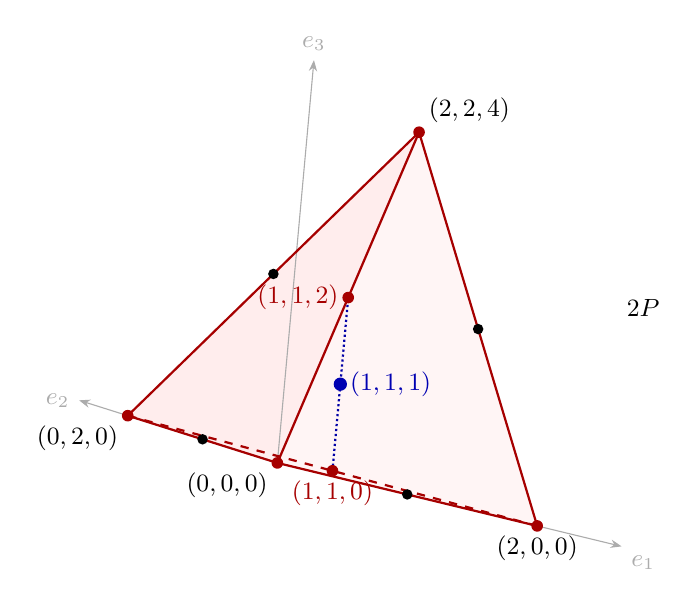
\begin{tikzpicture}[
        x={(1.65cm,-0.40cm)},y={(-0.95cm,0.30cm)},z={(0.10cm,1.10cm)},
        font=\small,line join=round,
        >={Stealth[length=4pt]}
    ]
        \coordinate (O) at (0,0,0);
        \coordinate (A) at (2,0,0);
        \coordinate (B) at (0,2,0);
        \coordinate (C) at (2,2,4);
        \coordinate (Qzero) at (1,1,0);
        \coordinate (Qone) at (1,1,1);
        \coordinate (Qtwo) at (1,1,2);
        \fill[red!4] (O)--(A)--(C)--cycle;
        \fill[red!7] (O)--(B)--(C)--cycle;
        \draw[->,gray!65] (O)--(2.65,0,0) node[below right] {$e_1$};
        \draw[->,gray!65] (O)--(0,2.65,0) node[left] {$e_2$};
        \draw[->,gray!65] (O)--(0,0,4.65) node[above] {$e_3$};
        \draw[red!65!black,thick,dashed] (A)--(B);
        \draw[red!65!black,thick] (O)--(A)--(C)--(B)--cycle;
        \draw[red!65!black,thick] (O)--(C);
        \draw[blue!65!black,densely dotted,thick] (Qzero)--(Qtwo);
        % The four unlabelled black dots are the other edge midpoints.
        \foreach \point in {(1,0,0),(0,1,0),(2,1,2),(1,2,2)}
            \fill[black] \point circle (1.9pt);
        \foreach \point in {O,A,B,C,Qzero,Qtwo}
            \fill[red!65!black] (\point) circle (2.1pt);
        \fill[blue!70!black] (Qone) circle (2.4pt);
        \node[below left] at (O) {$(0,0,0)$};
        \node[below] at (A) {$(2,0,0)$};
        \node[below left] at (B) {$(0,2,0)$};
        \node[above right] at (C) {$(2,2,4)$};
        \node[below,text=red!65!black] at (Qzero) {$(1,1,0)$};
        \node[right,text=blue!70!black] at (Qone) {$(1,1,1)$};
        \node[left,text=red!65!black] at (Qtwo) {$(1,1,2)$};
        \node at (2.65,0,2.75) {$2P$};
    \end{tikzpicture}
    \caption{All eleven lattice points of \(2P\), including
    the two edge midpoints \((2,1,2)\) and \((1,2,2)\).
    The highlighted collinear points satisfy
    \(2(1,1,1)=(1,1,0)+(1,1,2)\), yielding the homogeneous relation
    \(X_4^2=X_3X_5\) for the three corresponding coordinates.}
    \label{fig:oct19-diagram6}
\end{figure}

The complete map now targets \(\bP^{10}\). On the torus, the new
coordinate recovers the missing sign:
\[
    u=\frac{stu}{st}=\frac{X_4}{X_3}.
\]
The three highlighted collinear lattice points also give the
homogeneous equation
\[
    \boxed{X_4^2=X_3X_5.}
\]
This is one relation on the image, not a complete set of its equations.

To prove an embedding, we must also check the boundary charts.
Let \(v\) be any vertex of \(P\), and write
\[
    r_i=v_i-v\quad(i=1,2,3)
\]
for its differences to the other three vertices. Their determinant
has absolute value two, and
\[
    h_v=h-2v=\tfrac12(r_1+r_2+r_3)\in M.
\]
The half-open fundamental parallelepiped of the \(r_i\) contains
exactly the two lattice points \(0,h_v\). Subtracting integral
parts of the cone coefficients therefore gives
\[
    \Cone(P-v)\cap M
      =\bN r_1+\bN r_2+\bN r_3+\bN h_v.
\]
Each generator occurs among the normalized sections at the vertex
\(2v\) of \(2P\):
\[
    r_i=(v+v_i)-2v,\qquad h_v=h-2v,
    \qquad v+v_i,\ h\in2P\cap M.
\]
Thus the complete sections of \(2D_P\) generate every affine chart
coordinate ring. The vertex-chart criterion proves that
\[
    X_{\Sigma_P}\hookrightarrow\bP^{10}
\]
is a closed embedding. Hence \(D_P\) is ample but not very ample,
whereas \(2D_P\) is very ample. Doubling repairs the linear system;
it leaves the normal fan and the singularities of the variety unchanged.

% Lecture continuation: ampleness, the final board, and toric surfaces.
\section{Ampleness, normal fans, and projectivity}

Let \(X_\Sg\) be a normal complete toric variety and \(D\) a
torus-invariant Cartier divisor. Recall that \(D\) is ample when
\(nD\) is very ample for some integer \(n>0\). The fan formulation is
\[
    \boxed{D\text{ ample}
       \quad\Longleftrightarrow\quad
       P_D\text{ full dimensional and }\Sigma_{P_D}=\Sg.}
\]
Thus the polytope must recover the original fan, with all its cones
and walls.

For a basepoint-free divisor with full-dimensional \(P_D\), the
original fan \(\Sg\) refines the normal fan \(\Sigma_{P_D}\):
each cone of \(\Sg\) lies in a cone of \(\Sigma_{P_D}\).
The latter can be a \emph{coarser} fan, with fewer walls. Neighboring
cones can merge, and a ray of \(\Sg\) can lie in the interior of a
higher-dimensional cone of \(\Sigma_{P_D}\). The basepoint-free
hypothesis matters here. If \(P_D\) has smaller dimension, its normal
fan is considered in the quotient dual to
\(\operatorname{span}_{\bR}(P_D-P_D)\).

% Diagram 7: a triangular slice of a three-dimensional fan refinement.
\Needspace{9cm}
\begin{figure}[htbp]
    \centering
    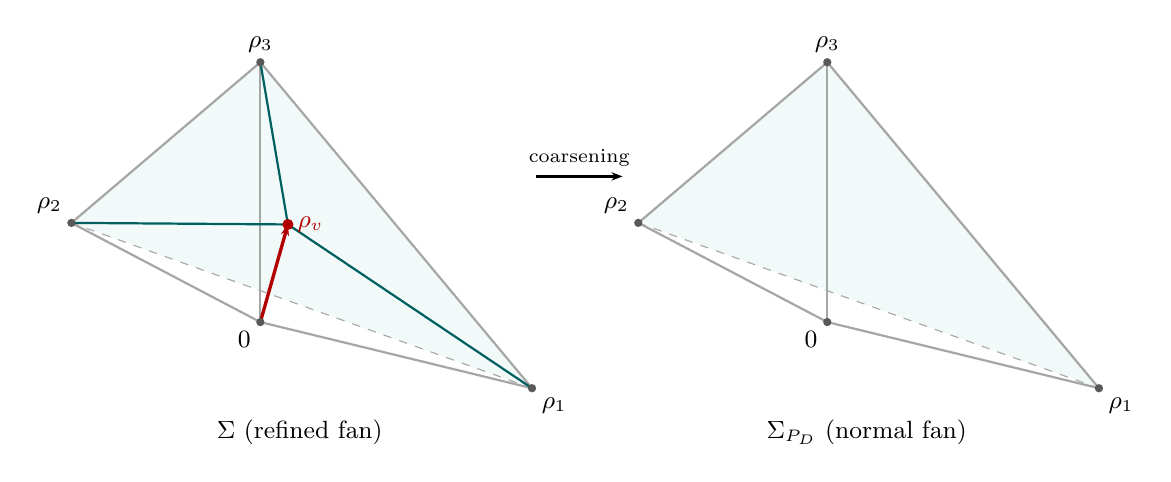
\begin{tikzpicture}[font=\small,line join=round,>={Stealth[length=4pt]}]
        \begin{scope}[
            xshift=-3.60cm,
            x={(1.15cm,-0.28cm)},y={(-0.80cm,0.42cm)},z={(0cm,1.10cm)}
        ]
            \coordinate (Ofine) at (0,0,0);
            \coordinate (Afine) at (3,0,0);
            \coordinate (Bfine) at (0,3,0);
            \coordinate (Cfine) at (0,0,3);
            \coordinate (Vfine) at (1,1,1);
            \fill[teal!5] (Afine)--(Bfine)--(Cfine)--cycle;
            \draw[gray!70,thick] (Ofine)--(Afine)--(Cfine)--(Bfine)--cycle;
            \draw[gray!70,thick] (Ofine)--(Cfine);
            \draw[gray!70,dashed] (Afine)--(Bfine);
            \draw[teal!75!black,thick]
                (Afine)--(Vfine)--(Bfine) (Vfine)--(Cfine);
            \draw[->,red!70!black,very thick] (Ofine)--(Vfine);
            \foreach \point in {Ofine,Afine,Bfine,Cfine}
                \fill[gray!70!black] (\point) circle (1.5pt);
            \fill[red!70!black] (Vfine) circle (2pt);
            \node[below left] at (Ofine) {$0$};
            \node[below right] at (Afine) {$\rho_1$};
            \node[above left] at (Bfine) {$\rho_2$};
            \node[above] at (Cfine) {$\rho_3$};
            \node[right,text=red!70!black] at (Vfine) {$\rho_v$};
        \end{scope}
        \begin{scope}[
            xshift=3.60cm,
            x={(1.15cm,-0.28cm)},y={(-0.80cm,0.42cm)},z={(0cm,1.10cm)}
        ]
            \coordinate (Ocoarse) at (0,0,0);
            \coordinate (Acoarse) at (3,0,0);
            \coordinate (Bcoarse) at (0,3,0);
            \coordinate (Ccoarse) at (0,0,3);
            \fill[teal!5] (Acoarse)--(Bcoarse)--(Ccoarse)--cycle;
            \draw[gray!70,thick] (Ocoarse)--(Acoarse)--(Ccoarse)--(Bcoarse)--cycle;
            \draw[gray!70,thick] (Ocoarse)--(Ccoarse);
            \draw[gray!70,dashed] (Acoarse)--(Bcoarse);
            \foreach \point in {Ocoarse,Acoarse,Bcoarse,Ccoarse}
                \fill[gray!70!black] (\point) circle (1.5pt);
            \node[below left] at (Ocoarse) {$0$};
            \node[below right] at (Acoarse) {$\rho_1$};
            \node[above left] at (Bcoarse) {$\rho_2$};
            \node[above] at (Ccoarse) {$\rho_3$};
        \end{scope}
        \draw[->,thick] (-0.10,1.85)--(1.00,1.85)
            node[midway,above,font=\scriptsize] {coarsening};
        \node at (-3.10,-1.40) {$\Sigma$ (refined fan)};
        \node at (4.10,-1.40) {$\Sigma_{P_D}$ (normal fan)};
    \end{tikzpicture}
    \caption{A triangular slice of one three-dimensional cone of the normal
    fan of a simplex. Adding the interior ray
    \(\rho_v=\mathbb{R}_{\geq0}(u_1+u_2+u_3)\) subdivides this cone into
    three cones; the other cones of the complete fan are unchanged.
    The identity lattice map induces the coarsening morphism
    \(X_\Sigma\longrightarrow X_{\Sigma_{P_D}}\).
    This is a schematic example, separate from the preceding tetrahedron.}
    \label{fig:oct19-diagram7}
\end{figure}

\subsection{Strict convexity remembers every wall}

Use the classroom sign convention from October 16:
\[
    q_\sigma=-m_\sigma,\qquad
    \psi_D(u)=\braket{q_\sigma}{u}\quad(u\in\sigma),
    \qquad\psi_D(u_\rho)=a_\rho.
\]
Basepoint freeness is equivalent to the maximum formula
\[
    \psi_D(u)=\max_{\sigma\in\Sg(\dim X)}
                       \braket{q_\sigma}{u}.
\]
Assume this convexity condition holds. If adjacent cones have the
same linear piece, the function does not
notice their common wall. Strict convexity requires a genuine bend
at every wall: its maximal domains of linearity must be exactly the
maximal cones of \(\Sg\). Equivalently, for every maximal cone
\(\sigma\),
\[
    \psi_D(u)=\braket{q_\sigma}{u}
       \quad\Longleftrightarrow\quad u\in\sigma.
\]
Here strict convexity is relative to the fan; the function is
still linear on each cone. We obtain
\[
    D\text{ ample}\quad\Longleftrightarrow\quad
    \psi_D\text{ strictly convex}.
\]
With the opposite support-function convention, one negates
\(\psi_D\) and uses a minimum instead; the geometric criterion is
unchanged.

\begin{Rmk}[The question about the canonical divisor]
    Being \(\bQ\)-Gorenstein means that the canonical divisor \(K_X\)
    is \(\bQ\)-Cartier: some positive integer multiple of \(K_X\)
    is Cartier. This is a condition on the canonical divisor, distinct
    from ampleness of a chosen divisor \(D\). The latter asks whether
    a positive multiple of \(D\) gives a projective embedding.
\end{Rmk}

\subsection{How to ask whether a toric variety is projective}

First ask for completeness: a projective variety is complete.
For a toric variety this means
\[
    |\Sg|=N_\bR.
\]
Over \(\bC\), this is equivalent to compactness in the complex
analytic topology. Next ask whether the fan admits an
\emph{integral strictly convex support function}. Such a function
produces an ample Cartier divisor. Hence
\[
    X_\Sg\text{ projective}
    \quad\Longleftrightarrow\quad
    \begin{gathered}
        \Sg\text{ is complete and admits an}\\
        \text{integral strictly convex support function}.
    \end{gathered}
\]
Completeness alone is insufficient in dimensions three and higher.
For surfaces, however, the second condition follows automatically.

\section{The surface dictionary}

The following discussion concerns normal toric surfaces. For the
calculations, return to the two-dimensional trapezoid from
Diagram~\ref{fig:oct19-diagram2}:
\[
    P=\Conv\{(0,0),(2,0),(1,1),(0,1)\}.
\]
Write \(D\) for its associated very ample divisor on
\(X_{\Sigma_P}\).

\begin{enumerate}
    \item \textbf{Completeness is equivalent to projectivity.}
    Every complete two-dimensional fan is the normal fan of a lattice
    polygon. Thus every normal complete toric surface is projective.

    The classroom picture is \emph{pitching a tent}: choose pole heights
    on the rays so that a piecewise-linear bedsheet bends strictly
    across every wall. This asserts that suitable heights
    \emph{exist}; arbitrary heights need not be convex.

    One construction explains the existence. List the primitive rays
    \(u_i=(a_i,b_i)\) in counterclockwise order. Completeness gives
    positive rational numbers \(\lambda_i\) with
    \(\sum_i\lambda_i u_i=0\): express each \(-u_i\) as a nonnegative
    rational combination of rays and sum the resulting relations.
    Clear denominators. The integral edge vectors
    \[
        \lambda_i(b_i,-a_i)
    \]
    then form a closed convex polygonal chain. Its inward normals
    are precisely the \(u_i\), so the resulting lattice polygon has
    the prescribed normal fan.

    \item \textbf{Smoothness is visible at the vertices.}
    At a vertex \(p\), take the two \emph{primitive} lattice vectors
    \(u,v\in M\) pointing from \(p\) along its adjacent edges. The
    corresponding affine chart is smooth exactly when
    \[
        |\det(u,v)|=1.
    \]
    In other words, these directions must form a basis of \(M\).
    The surface is smooth when this holds at every vertex.
    These are directions in the tangent cone in \(M_\bR\); its dual
    is the corresponding normal fan cone in \(N_\bR\).

    % Final board, middle column: primitive directions and determinant.
    \begin{figure}[htbp]
        \centering
        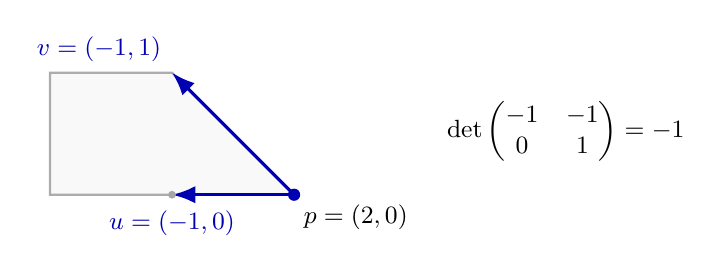
\begin{tikzpicture}[>=Latex,font=\small]
            \begin{scope}[x=1.55cm,y=1.55cm]
                \fill[gray!5] (0,0)--(2,0)--(1,1)--(0,1)--cycle;
                \draw[gray!65,thick] (0,0)--(2,0)--(1,1)--(0,1)--cycle;
                \fill[blue!70!black] (2,0) circle (2.2pt);
                \node[below right] at (2,0) {$p=(2,0)$};
                \draw[->,blue!70!black,very thick] (2,0)--(1,0);
                \node[below,blue!70!black] at (1,-0.05) {$u=(-1,0)$};
                \draw[->,blue!70!black,very thick] (2,0)--(1,1)
                    node[above left] {$v=(-1,1)$};
                \fill[gray!70] (1,0) circle (1.4pt);
            \end{scope}
            \node at (6.55,0.8)
                {$\displaystyle
                    \det\begin{pmatrix}-1&-1\\0&1\end{pmatrix}=-1$};
        \end{tikzpicture}
        \caption{The primitive edge directions at \(p=(2,0)\)
        form a lattice basis. The full bottom edge has length two,
        but its primitive direction is \((-1,0)\).}
        \label{fig:oct19-diagram8}
    \end{figure}

    At the marked vertex, \(u=(-1,0)\) and \(v=(-1,1)\) give
    determinant \(-1\). The other three vertices also pass the
    primitive-vector test, so this surface is smooth. Using the full
    bottom-edge vector \((-2,0)\) would give the wrong smoothness test.

    \item \textbf{Intersection with an invariant curve is an edge length.}
    For a ray \(\rho\), let \(F_\rho\) be the edge of \(P_D\)
    with primitive inward normal \(u_\rho\). The corresponding
    torus-invariant divisor \(D_\rho\) is a curve, and
    \[
        \boxed{D\cdot D_\rho=\operatorname{Length}_M(F_\rho).}
    \]
    For endpoints \(p,q\), write \(q-p=\ell w\) with \(w\) primitive;
    then the lattice length is \(\ell\), or equivalently
    \(|F_\rho\cap M|-1\). The length is measured in the lattice,
    not by Euclidean distance.

    % Final board, right column: color-matched fan rays and polygon edges.
    \begin{figure}[htbp]
        \centering
        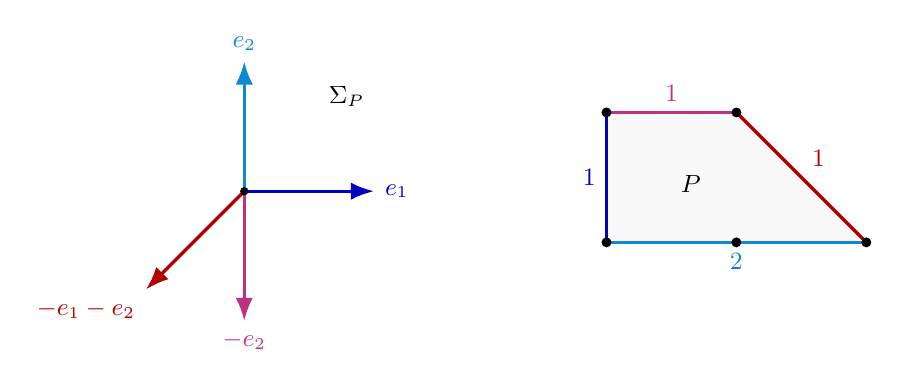
\begin{tikzpicture}[>=Latex,font=\small]
            \begin{scope}[shift={(1.8,1.65)},x=1cm,y=1cm]
                \draw[->,blue!75!black,very thick] (0,0)--(1.65,0)
                    node[right] {$e_1$};
                \draw[->,cyan!70!blue,very thick] (0,0)--(0,1.65)
                    node[above] {$e_2$};
                \draw[->,red!70!black,very thick] (0,0)--(-1.25,-1.25)
                    node[below left] {$-e_1-e_2$};
                \draw[->,magenta!75!black,very thick] (0,0)--(0,-1.65)
                    node[below] {$-e_2$};
                \fill (0,0) circle (1.5pt);
                \node at (1.3,1.2) {$\Sigma_P$};
            \end{scope}
            \begin{scope}[shift={(6.4,1)},x=1.65cm,y=1.65cm]
                \fill[gray!5] (0,0)--(2,0)--(1,1)--(0,1)--cycle;
                \draw[blue!75!black,very thick] (0,0)--(0,1)
                    node[midway,left] {$1$};
                \draw[cyan!70!blue,very thick] (0,0)--(2,0)
                    node[midway,below] {$2$};
                \draw[magenta!75!black,very thick] (0,1)--(1,1)
                    node[midway,above] {$1$};
                \draw[red!70!black,very thick] (1,1)--(2,0)
                    node[midway,above right] {$1$};
                \foreach \p in {(0,0),(1,0),(2,0),(1,1),(0,1)}
                    \fill[black] \p circle (1.8pt);
                \node at (0.65,0.45) {$P$};
            \end{scope}
        \end{tikzpicture}
        \caption{Matching colors identify a fan ray with the polygon
        edge whose inward normal it gives. The numbers on the edges
        are their lattice lengths, hence the intersections
        \(D\cdot D_\rho\).}
        \label{fig:oct19-diagram9}
    \end{figure}

    The four intersection numbers are
    \[
        \begin{array}{c|c|c}
            u_\rho&F_\rho&D\cdot D_\rho\\ \hline
            \textcolor{blue!75!black}{e_1}&r=0&1\\
            \textcolor{cyan!70!blue}{e_2}&q=0&2\\
            \textcolor{magenta!75!black}{-e_2}&q=1&1\\
            \textcolor{red!70!black}{-e_1-e_2}&r+q=2&1
        \end{array}
    \]
    Thus dark blue gives \(1\), light blue gives \(2\), pink gives
    \(1\), and red gives \(1\), as on the board.

    \item \textbf{The degree is twice the lattice area.}
    If a very ample divisor \(D\) embeds the surface by \(\vf_D\),
    two general hyperplanes pull back to divisors in \(|D|\).
    Their intersection number is the degree of the image:
    \[
        \deg\vf_D(X_\Sg)=D^2
           =2\operatorname{Area}_M(P_D).
    \]
    Here a fundamental lattice parallelogram has area \(1\).
    The factor \(2=2!\) converts that area into normalized lattice
    volume.

    One way to see the formula is to compare leading coefficients:
    lattice-point counting gives
    \[
        h^0(X_\Sg,\cO(kD))
           =|kP_D\cap M|
           =\operatorname{Area}_M(P_D)k^2+O(k),
    \]
    while the Hilbert polynomial has leading term
    \(\tfrac12D^2k^2\).
    For our trapezoid,
    \[
        \operatorname{Area}_M(P)=\frac{2+1}{2}\cdot1=\frac32,
        \qquad\boxed{D^2=3.}
    \]
    Therefore the surface embedded in \(\bP^4\) by the five
    monomial sections has degree \(3\).
\end{enumerate}

% Final classroom discussion: the ruled surface and divisor classes in Diagram 9.
\section{The Hirzebruch surface behind Diagram 9}

The surface in Diagram~\ref{fig:oct19-diagram9} is the first Hirzebruch
surface
\[
    X=X_{\Sigma_P}\isom\bF_1\isom\Bl_p\bP^2.
\]
The following names identify the four boundary curves by their colors
and primitive ray generators:
\[
    \begin{array}{c|c|c}
        \text{curve}&u_\rho&\text{geometric role}\\ \hline
        \textcolor{blue!75!black}{F}&(1,0)&\text{fiber}\\
        \textcolor{cyan!70!blue}{B}&(0,1)&\text{positive section}\\
        \textcolor{red!70!black}{F'}&(-1,-1)&\text{fiber}\\
        \textcolor{magenta!75!black}{E}&(0,-1)&\text{negative section}
    \end{array}
\]
There is a ruling \(\pi:\bF_1\to\bP^1\), given on the torus by
\((s,t)\mapsto s\). Its two invariant fibers are \(F,F'\), over
\(0,\infty\), respectively. The curves \(E,B\) are disjoint sections,
each meeting every fiber once. The curve \(E\) is also the exceptional
curve of the blowup.

% Continuation of Diagram 9: sections and fibers on the ruled surface.
\begin{center}
    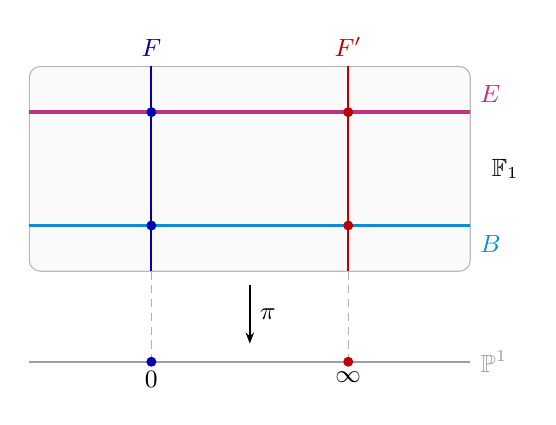
\begin{tikzpicture}[font=\small,>={Stealth[length=4pt]}]
        \fill[gray!4] (-2.80,-1.30) rectangle (2.80,1.30);
        \draw[gray!55,rounded corners=4pt]
            (-2.80,-1.30) rectangle (2.80,1.30);
        \node[right] at (2.95,0) {$\mathbb{F}_1$};
        % Disjoint sections; the sheet is only a schematic of the surface.
        \draw[magenta!75!black,very thick] (-2.80,0.72)--(2.80,0.72);
        \node[above right,text=magenta!75!black] at (2.80,0.72) {$E$};
        \draw[cyan!75!blue,very thick] (-2.80,-0.72)--(2.80,-0.72);
        \node[below right,text=cyan!75!blue] at (2.80,-0.72) {$B$};
        % Two distinct fibers each meet each section once.
        \draw[blue!70!black,thick] (-1.25,-1.30)--(-1.25,1.30);
        \node[above,text=blue!70!black] at (-1.25,1.30) {$F$};
        \draw[red!75!black,thick] (1.25,-1.30)--(1.25,1.30);
        \node[above,text=red!75!black] at (1.25,1.30) {$F'$};
        \foreach \height in {-0.72,0.72} {
            \fill[blue!70!black] (-1.25,\height) circle (1.8pt);
            \fill[red!75!black] (1.25,\height) circle (1.8pt);
        }
        \draw[gray!60,densely dashed] (-1.25,-1.30)--(-1.25,-2.45);
        \draw[gray!60,densely dashed] (1.25,-1.30)--(1.25,-2.45);
        \draw[->,thick] (0,-1.48)--(0,-2.22)
            node[midway,right] {$\pi$};
        \draw[thick,gray!75] (-2.80,-2.45)--(2.80,-2.45)
            node[right] {$\mathbb{P}^1$};
        \fill[blue!70!black] (-1.25,-2.45) circle (1.8pt);
        \fill[red!75!black] (1.25,-2.45) circle (1.8pt);
        \node[below] at (-1.25,-2.45) {$0$};
        \node[below] at (1.25,-2.45) {$\infty$};
    \end{tikzpicture}

    \smallskip
    {\small\textbf{Continuing Diagram 9.}
    Schematic of the ruling \(\pi:\mathbb{F}_1\to\mathbb{P}^1\).
    The sections \(E\) and \(B\) are disjoint; the fibers
    \(F=\pi^{-1}(0)\) and \(F'=\pi^{-1}(\infty)\)
    each meet each section once.\par}
\end{center}

\subsection{The class group relations come from characters}

For a toric character, the principal divisor formula is
\[
    \divisor(\chi^m)=
       \sum_\rho\braket{m}{u_\rho}D_\rho.
\]
Apply it to \(s=\chi^{(1,0)}\) and \(t=\chi^{(0,1)}\):
\[
    \divisor(s)=F-F',\qquad
    \divisor(t)=B-F'-E.
\]
Principal divisors represent zero in the divisor class group.
Consequently,
\[
    F'\sim F,\qquad B\sim E+F.
\]
The board's formula \(B=E+F\) is this equality of divisor classes;
\(\sim\) denotes linear equivalence.

The invariant divisors generate \(\Cl(X)\), and the character
divisors give all their relations. Explicitly,
\[
    \Cl(X)=
    \frac{\bZ F\oplus\bZ B\oplus\bZ F'\oplus\bZ E}
         {\langle F-F',\,B-F'-E\rangle}
    \isom\bZ[F]\oplus\bZ[E].
\]
Eliminating \(F'\) and \(B\) leaves the two free generators
\([F],[E]\). Since \(X\) is smooth, every Weil divisor is Cartier,
so
\[
    \boxed{\Pic(\bF_1)=\Cl(\bF_1)
                  \isom\bZ[F]\oplus\bZ[E].}
\]
Intersection numbers depend only on these classes and are bilinear.

\subsection{Recovering the intersection table}

Distinct fibers are disjoint, and \(F'\sim F\), so
\[
    F^2=F\cdot F'=0.
\]
Each section meets a fiber transversely once:
\[
    E\cdot F=1,\qquad B\cdot F=1.
\]
The sections \(E,B\) are disjoint. Substituting \(B\sim E+F\)
therefore gives
\[
    0=E\cdot B=E\cdot(E+F)=E^2+1,
    \qquad E^2=-1.
\]
Finally,
\[
    B^2=(E+F)^2=-1+2+0=1.
\]
Thus the board's list is
\[
    \boxed{F^2=0,\quad E^2=-1,\quad B^2=1,\quad
           E\cdot B=0,\quad E\cdot F=B\cdot F=1.}
\]
In the ordered basis \(([F],[E])\), the intersection matrix is
\[
    \begin{pmatrix}0&1\\1&-1\end{pmatrix}.
\]
The schematic picture supplies the intersections of distinct curves;
linear equivalence then determines the self-intersections.

\subsection{Recovering the four edge lengths in Diagram 9}

The divisor coefficients on the fan are \(0,0,2,1\), in the order
\((F,B,F',E)\). Thus the polygon's actual invariant divisor is
\[
    D=2F'+E,\qquad D\sim2F+E.
\]
Using the intersection table, we recover every colored edge length:
\[
    \begin{aligned}
        D\cdot F  &=(2F+E)\cdot F=1
                      &&\text{(dark blue)},\\
        D\cdot B  &=(2F+E)\cdot B=2
                      &&\text{(light blue)},\\
        D\cdot E  &=(2F+E)\cdot E=2-1=1
                      &&\text{(pink)},\\
        D\cdot F' &=D\cdot F=1
                      &&\text{(red)}.
    \end{aligned}
\]
In particular, \(D\cdot E=1\) and \(E^2=-1\) are different products.
The first is the degree of the chosen line bundle along \(E\);
the second is the degree of \(\cO_X(E)|_E\).

The self-intersection of the embedding divisor is
\[
    D^2=(2F+E)^2=4F^2+4F\cdot E+E^2=3,
\]
agreeing with twice the area of the trapezoid.
If \(H\) is the pullback of the line class under
\(\Bl_p\bP^2\to\bP^2\), then \(B\sim H\) and \(F\sim H-E\).
Consequently
\[
    D\sim2F+E\sim2H-E,
\]
connecting this example with the earlier five-section embedding
of the blowup into \(\bP^4\).

\begin{Rmk}[The other Hirzebruch surfaces]
    For \(r\geq0\), replacing the red ray by \((-1,-r)\) gives
    the fan of \(\bF_r\). If \(E\) denotes the section of
    self-intersection \(-r\), and \(F\) a fiber, then
    \[
        \Pic(\bF_r)=\Cl(\bF_r)=\bZ[E]\oplus\bZ[F],
        \qquad B\sim E+rF,
    \]
    \[
        F^2=0,\qquad E\cdot F=1,\qquad E^2=-r,
        \qquad B^2=r,\qquad E\cdot B=0.
    \]
    Hence a class \(aE+bF\) has square \(2ab-ra^2\).
    The Hirzebruch index \(r\) records the self-intersection of \(E\);
    the degree of a projective embedding also depends on the chosen
    divisor. Our surface is \(\bF_1\), with embedding degree \(3\).
\end{Rmk}

% Closing transcript and board photographs: bundle restriction and the star fan.
\section{Intersections by restricting the line bundle}

Let \(X\) be a smooth projective surface, \(C\subset X\) a smooth
complete curve, and \(L=\cO_X(D)\). The line bundle always restricts
to \(L|_C\), and
\[
    \boxed{D\cdot C=\deg(L|_C).}
\]
When \(L\) has a nonzero regular section, choose one,
\(\widetilde{s}\). Its zero divisor
\(Z(\widetilde{s})\) is linearly equivalent to \(D\).
Its zero set is where the graph of the section meets the zero
section of the bundle.

If \(C\) is not a component of \(Z(\widetilde{s})\), then
\(\widetilde{s}|_C\not\equiv0\), and its zeros are the intersection
with \(C\). Thus
\[
    D\cdot C
       =\sum_{p\in C\cap Z(\widetilde{s})}
                         \ord_p(\widetilde{s}|_C).
\]
An intersection transverse to \(C\) contributes \(1\); otherwise its
multiplicity must be counted.

If \(C\) is a component of \(Z(\widetilde{s})\), the restricted
section is identically zero. The line bundle \(L|_C\) still exists,
but this section does not give a finite divisor on \(C\).
When a regular replacement is available, choose one whose restriction
is nonzero. A basepoint-free system guarantees such a choice;
over \(\bC\), a general section has
simple zeros on \(C\). In our example \(D\) is very ample, so this
choice is available.

\Needspace{9cm}
% Diagram 10: restricting a line bundle and a section to a curve.
\begin{figure}[htbp]
    \centering
    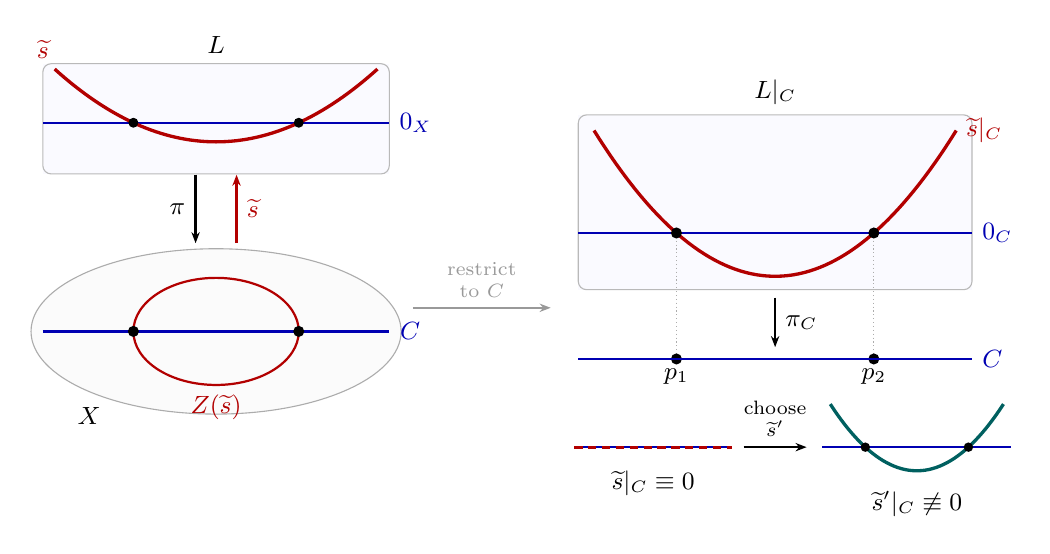
\begin{tikzpicture}[font=\small,>={Stealth[length=4pt]},line join=round]
        % A schematic slice of L shows its zero section and a section graph.
        \fill[blue!2] (-5.80,2.00) rectangle (-1.40,3.40);
        \draw[gray!55,rounded corners=3pt] (-5.80,2.00) rectangle (-1.40,3.40);
        \node[above] at (-3.60,3.40) {$L$};
        \draw[blue!70!black,thick] (-5.80,2.65)--(-1.40,2.65)
            node[right] {$0_X$};
        \draw[red!70!black,very thick,domain=-5.65:-1.55,samples=65]
            plot (\x,{2.65+0.22*((\x+3.60)*(\x+3.60)-1.1025)});
        \fill[black] (-4.65,2.65) circle (1.8pt);
        \fill[black] (-2.55,2.65) circle (1.8pt);
        \node[above left,text=red!70!black] at (-5.60,3.34) {$\widetilde{s}$};
        \draw[->,thick] (-3.86,1.99)--(-3.86,1.12)
            node[midway,left] {$\pi$};
        \draw[->,red!70!black,thick] (-3.34,1.12)--(-3.34,1.99)
            node[midway,right] {$\widetilde{s}$};
        \fill[gray!3] (-3.60,0) ellipse[x radius=2.35,y radius=1.05];
        \draw[gray!65] (-3.60,0) ellipse[x radius=2.35,y radius=1.05];
        \node[below left] at (-4.94,-0.84) {$X$};
        \draw[blue!70!black,very thick] (-5.80,0)--(-1.40,0)
            node[right] {$C$};
        \draw[red!70!black,thick] (-3.60,0) ellipse[x radius=1.05,y radius=0.68];
        \node[below,text=red!70!black] at (-3.60,-0.68) {$Z(\widetilde{s})$};
        \fill[black] (-4.65,0) circle (2pt);
        \fill[black] (-2.55,0) circle (2pt);
        \draw[->,gray!80,thick] (-1.10,0.30)--(0.65,0.30)
            node[midway,above,align=center,font=\scriptsize]
            {restrict\\to $C$};
        % A ribbon represents L|_C; the blue line is its zero section.
        \fill[blue!2] (1.00,0.53) rectangle (6.00,2.75);
        \draw[gray!55,rounded corners=3pt] (1.00,0.53) rectangle (6.00,2.75);
        \node[above] at (3.50,2.75) {$L|_C$};
        \draw[blue!70!black,thick] (1.00,1.25)--(6.00,1.25)
            node[right] {$0_C$};
        \draw[red!70!black,very thick,domain=1.2:5.8,samples=70]
            plot (\x,{0.70+0.35*(\x-3.50)*(\x-3.50)});
        \node[right,text=red!70!black] at (5.80,2.55) {$\widetilde{s}|_C$};
        \foreach \point in {2.24643,4.75357} {
            \draw[gray!65,densely dotted] (\point,1.25)--(\point,-0.35);
            \fill[black] (\point,1.25) circle (2pt);
            \fill[black] (\point,-0.35) circle (2pt);
        }
        \draw[->,thick] (3.50,0.43)--(3.50,-0.20)
            node[midway,right] {$\pi_C$};
        \draw[blue!70!black,thick] (1.00,-0.35)--(6.00,-0.35)
            node[right] {$C$};
        \node[below] at (2.24643,-0.35) {$p_1$};
        \node[below] at (4.75357,-0.35) {$p_2$};
        % A section vanishing identically gives no finite zero divisor on C.
        \draw[blue!70!black,thick] (0.95,-1.47)--(2.95,-1.47);
        \draw[red!70!black,very thick,densely dashed] (0.95,-1.47)--(2.95,-1.47);
        \node[below] at (1.95,-1.65) {$\widetilde{s}|_C\equiv0$};
        \draw[->,thick] (3.10,-1.47)--(3.90,-1.47)
            node[midway,above,align=center,font=\scriptsize]
            {choose\\$\widetilde{s}'$};
        \draw[blue!70!black,thick] (4.10,-1.47)--(6.50,-1.47);
        \draw[teal!75!black,very thick,domain=4.2:6.4,samples=50]
            plot (\x,{-1.77+0.70*(\x-5.30)*(\x-5.30)});
        \fill[black] (4.64535,-1.47) circle (1.7pt);
        \fill[black] (5.95465,-1.47) circle (1.7pt);
        \node[below] at (5.30,-1.90) {$\widetilde{s}'|_C\not\equiv0$};
    \end{tikzpicture}
    \caption{Restricting a line bundle and a section to a smooth projective
    curve. When \(\widetilde{s}|_C\not\equiv0\), its zero divisor is finite and is
    obtained by restricting \(Z(\widetilde{s})\) to \(C\), with multiplicities.
    The lower sketches contrast a section vanishing identically on \(C\)
    with a replacement section whose restriction is nonzero.
    The bundle panels are schematic slices; the crossings do not assert transversality.}
    \label{fig:oct19-diagram10}
\end{figure}

\subsection{Changing the section adds a principal divisor}

Any two nonzero rational sections of the same line bundle differ
by a nonzero rational function:
\[
    \widetilde{s}'=g\widetilde{s},\qquad
    \divisor(\widetilde{s}')
       =\divisor(\widetilde{s})+\divisor(g).
\]
This is the meaning of moving a divisor within its linear equivalence
class. The line bundle remains the same.

For an arbitrary line bundle, a regular replacement avoiding \(C\)
need not exist. One can instead choose a rational section with neither
a zero nor a pole along the generic point of \(C\). Its restriction
is a nonzero rational section of \(L|_C\), and the degree is the
number of zeros \emph{minus} the number of poles, with multiplicities.
Multiplication by a rational function produces another regular global
section precisely when its resulting section divisor is effective.
The toric choices below satisfy this condition.

\section{Restricting to a torus-invariant curve}

Continue with the fan and curve names from Diagram~\ref{fig:oct19-diagram9}:
\[
    F=D_{(1,0)},\quad B=D_{(0,1)},\quad
    F'=D_{(-1,-1)},\quad E=D_{(0,-1)},\qquad D=2F'+E.
\]
For a ray \(\rho\), the one-dimensional orbit is
\(O(\rho)\isom\bC^\times\). Its \emph{closure}
\[
    C=V(\rho)=D_\rho\isom\bP^1
\]
is the complete invariant curve used in the intersection calculation.

The fan of \(C\) is obtained in two steps: keep the cones containing
\(\rho\), then pass to the quotient lattice
\[
    N_\rho=N/\bZ u_\rho.
\]
Here \(u_\rho\) is primitive. The images of those cones form the
star fan
\[
    \Sigma_C=
    \set{\overline{\sigma}:\rho\subseteq\sigma\in\Sg}.
\]
In this surface example it is the complete one-dimensional fan with
two rays. Curves corresponding to rays outside this star need not
contribute, even if their vectors have nonzero images in the quotient.

\subsection{The coefficient on the chosen curve is already zero}

First take \(C=F\), the dark-blue curve. Its coefficient in
\(D=2F'+E\) is \(0\), so the canonical section \(s_D\) does not
vanish identically on \(F\). The two maximal cones containing its ray
are
\[
    \Cone(e_1,e_2),\qquad \Cone(-e_2,e_1).
\]
The quotient map is \(q(a,b)=b\). Its neighboring rays give
\[
    e_2\longmapsto1,\qquad -e_2\longmapsto-1.
\]
Their divisor coefficients are \(0\) and \(1\). Therefore
\[
    D|_F=[E\cap F],\qquad
    L|_F\isom\cO_{\bP^1}(1),\qquad D\cdot F=1.
\]
The red curve \(F'\) is disjoint from \(F\). Although its vector
\((-1,-1)\) also maps to \(-1\), its cones are not in this star:
projecting all rays would incorrectly include it.

\Needspace{8cm}
% Restriction to C=F=V(e_1): coefficient of F is already zero.
\begin{figure}[htbp]
    \centering
    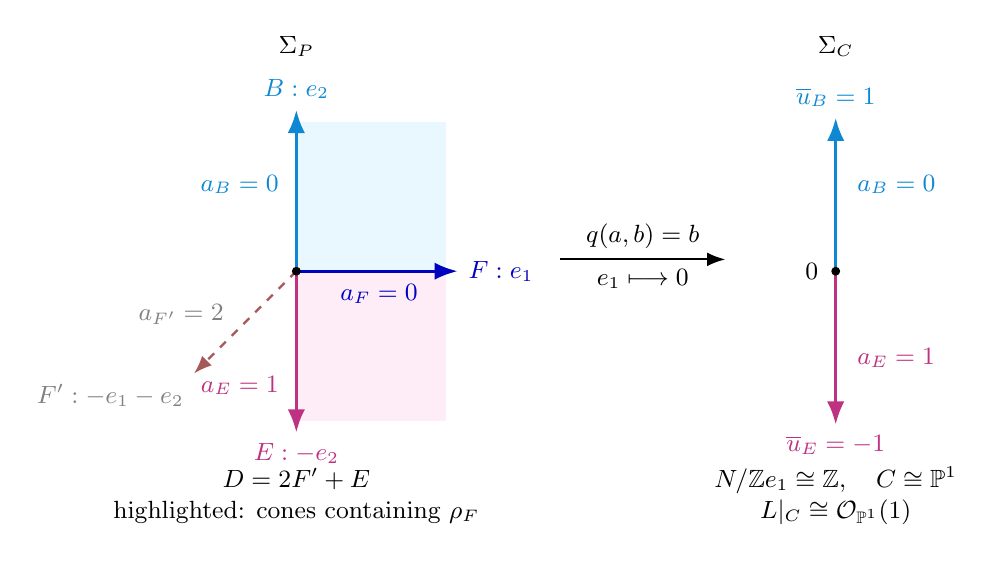
\begin{tikzpicture}[>=Latex,font=\small,line join=round]
        % Only the two maximal cones containing rho_F are highlighted.
        \fill[cyan!9] (0,0) rectangle (1.9,1.9);
        \fill[magenta!7] (0,0) rectangle (1.9,-1.9);
        \draw[->,blue!75!black,very thick] (0,0)--(2.05,0)
            node[right] {$F:e_1$};
        \draw[->,cyan!70!blue,very thick] (0,0)--(0,2.05)
            node[above] {$B:e_2$};
        \draw[->,magenta!75!black,very thick] (0,0)--(0,-2.05)
            node[below] {$E:-e_2$};
        \draw[->,red!30!gray,thick,dashed] (0,0)--(-1.3,-1.3)
            node[below left,text=gray] {$F':-e_1-e_2$};
        \fill (0,0) circle (1.6pt);
        \node[blue!75!black,below] at (1.05,-0.05) {$a_F=0$};
        \node[cyan!70!blue,left] at (-0.1,1.1) {$a_B=0$};
        \node[magenta!75!black,left] at (-0.1,-1.45) {$a_E=1$};
        \node[gray,left] at (-0.8,-0.55) {$a_{F'}=2$};
        \node at (0,2.85) {$\Sigma_P$};
        \node[align=center] at (0,-2.85)
            {$D=2F'+E$\\highlighted: cones containing $\rho_F$};

        \draw[->,thick] (3.35,0.15)--(5.45,0.15)
            node[midway,above] {$q(a,b)=b$}
            node[midway,below] {$e_1\longmapsto0$};

        \begin{scope}[shift={(6.85,0)}]
            \draw[->,cyan!70!blue,very thick] (0,0)--(0,1.95)
                node[above] {$\overline{u}_B=1$};
            \draw[->,magenta!75!black,very thick] (0,0)--(0,-1.95)
                node[below] {$\overline{u}_E=-1$};
            \fill (0,0) circle (1.6pt);
            \node[left] at (-0.1,0) {$0$};
            \node[cyan!70!blue,right] at (0.15,1.1) {$a_B=0$};
            \node[magenta!75!black,right] at (0.15,-1.1) {$a_E=1$};
            \node at (0,2.85) {$\Sigma_C$};
            \node[align=center] at (0,-2.85)
                {$N/\bZ e_1\isom\bZ,\quad C\isom\bP^1$\\
                 $L|_C\isom\cO_{\bP^1}(1)$};
        \end{scope}
    \end{tikzpicture}
    \caption{Restricting $L=\cO(D)$ to the dark-blue invariant curve
    $C=F=V(\rho_F)$. Its fan is obtained by taking the cones containing
    $\rho_F$ and passing to $N/\bZ e_1$. Since $a_F=0$, the neighboring
    coefficients $a_B=0$ and $a_E=1$ descend directly: the restricted
    divisor is one point on $\bP^1$, so $\deg L|_C=1$.
    The curve corresponding to the greyed red ray is disjoint from $C$
    and contributes nothing.}
    \label{fig:oct19-diagram11}
\end{figure}

\subsection{Removing a component before restricting}

Now take \(C=F'\), whose coefficient in \(D\) is \(2\).
The original section \(s_D\) vanishes identically on \(C\).
Use either of the following sections of the same line bundle:
\[
    \widetilde{s}_1=st\,s_D,\qquad
    \widetilde{s}_2=s^2s_D.
\]
The principal-divisor relations from the previous section give
\[
    \begin{aligned}
        A_1:=D+\divisor(st)&=F+B,\\
        A_2:=D+\divisor(s^2)&=2F+E.
    \end{aligned}
\]
Both divisors are effective, and neither contains \(F'\).
Their coefficients, in the original fan order, are
\[
    \begin{array}{c|cccc}
        &F&B&F'&E\\ \hline
        D&0&0&2&1\\
        A_1&1&1&0&0\\
        A_2&2&0&0&1
    \end{array}
\]

This is what the board's linear adjustments mean. In the classroom
convention \(\psi_D(u_\rho)=a_\rho\),
\[
    \psi_{D+\divisor(\chi^m)}(u)
       =\psi_D(u)+\braket{m}{u}.
\]
Writing \(u=(x,y)\), multiplication by \(st\) adds \(x+y\);
multiplication by \(s^2\) adds \(2x\). Both linear forms have value
\(-2\) at \((-1,-1)\), so the new coefficient there is \(0\).
The relevant linear pieces now annihilate that ray and descend to
the quotient \emph{on its star}.

For \(C=F'\), the quotient map is \(q'(a,b)=b-a\).
Again \(B\) maps to \(+1\) and \(E\) to \(-1\); the disjoint fiber
\(F\) contributes nothing. Set
\[
    p_B=B\cap F',\qquad p_E=E\cap F'.
\]
Then the two restrictions are
\[
    A_1|_{F'}=p_B,\qquad A_2|_{F'}=p_E.
\]
Their coefficient pairs on the quotient fan are \((1,0)\) and
\((0,1)\), respectively. Each is a point divisor on \(\bP^1\), so
both represent the same line bundle of degree \(1\).
Indeed, the quotient character \(z=(t/s)|_{F'}\) satisfies
\[
    \divisor_{F'}(z)=p_B-p_E.
\]
Thus the two choices differ by a principal divisor on the curve,
just as the two sections differ by \(t/s\).

\subsection{The restricted polytope is the corresponding edge}

The edge of \(P_D\) dual to \(F'\) is
\[
    G=\set{(r,q)\in P_D:r+q=2}
      =[(2,0),(1,1)].
\]
The two endpoints index the sections \(s^2s_D\) and \(st\,s_D\);
their restrictions to \(F'\) are not identically zero.

Changing the divisor by \(\divisor(\chi^m)\) translates its
polytope by \(-m\). The lattice of characters on \(F'\) is
\[
    M\cap(-1,-1)^\perp=\bZ(-1,1).
\]
In this rank-one lattice, the two choices above give
\[
    \begin{aligned}
        G-(1,1)&=[(1,-1),(0,0)]\isom[-1,0],\\
        G-(2,0)&=[(0,0),(-1,1)]\isom[0,1].
    \end{aligned}
\]
These intervals differ by a lattice translation and both have length
\(1\). This is the polytope version of the same calculation:
\[
    \boxed{D\cdot F'=\deg(L|_{F'})
          =\operatorname{Length}_M(G)=1.}
\]

\begin{Rmk}[A negative degree requires poles]
    The distinction between regular and rational sections also explains
    \(E^2=-1\). For the line bundle \(\cO_X(E)\), the original
    section vanishes on \(E\). Since
    \[
        E+\divisor(t)=B-F',
    \]
    a rational replacement restricts to
    \(-[E\cap F']\): \(B\) is disjoint from \(E\), while \(F'\)
    meets it once. There is one pole and no zero, giving degree
    \(-1\). A nonzero regular section of \(\cO_X(E)|_E\) could not
    have this negative degree.
\end{Rmk}

\end{document}
